\subsection{Block Processing}
Block processing is where the CPU processes the data blocks already stored in memory, together
without streaming more data. This is usually done with the data in vector form, see Intel AVX
instructions and ARM Neon intrinsics. An example of block processing could be a moving average
filter (MAF). For the moving average filter once it has been applied to the input data the output
must be stored in a separate memory section. This can pose issues in moving within memory and
between memory and peripherals.

\subsection{Unbuffered Data Transfer}
Unbuffered transfer is when no buffer is implemented on the input of data, this can cause
synchronization issues as both the sender and receiver need to be aware of the when the data is
transferred. A diagram of this is shown in Figure \ref{fig:unbuffered}\\

\noindent There are two methods for implementing unbuffered transfer, the first is to use
\textit{Polling}. Polling can waste CPU cycles as the CPU will have to reguarly check if data is
available. This can be somewhat mitigated through the use of the second method, \textit{Interrupts}
this method ensures that data can be transferred once it is available however, there can be
significant overhead created due to the context switch required to service the interrupt.

\begin{figure}[H]
\begin{center}
    \begin{circuitikz}
        \ctikzset{multipoles/thickness=3}
        \ctikzset{multipoles/dipchip/width=2.5}
    
        \draw (0,0) node[dipchip, num pins=6, hide numbers, no topmark, external pins
       width=0](shift) {8-bit shift register};

        \draw (0,-3) node[dipchip, num pins=6, hide numbers, no topmark, external pins
       width=0](framecount) {3-bit frame counter};

        \draw (framecount.bpin 2) ++(0,0.1) -- ++(0.1,-0.1) -- ++(-0.1,-0.1);
        \draw (shift.bpin 2) ++(0,0.1) -- ++(0.1,-0.1) -- ++(-0.1,-0.1);

        \draw (framecount.bpin 2) ++(-1.5,0) node[not port](invert){};
        
        \draw (invert.in) -- ++(-0.5,0) node[left] {SCK};
        \draw (invert.out) -- ++(0.5,0) |- (shift.bpin 2);
        \draw (invert.out) -- (framecount.bpin 2);
        
        \draw (shift.bpin 1) -- ++(-1.5,0) node[left] {MOSI};

        \draw (shift.bpin 1) node[right] {\tiny D};
        \draw (shift.s) node[above] {\tiny Q(0:7)};
        \draw[line width=3pt] (shift.s) |- (4,-1.5) node[right] {SPIDATA};
        \draw (framecount.bpin 6) -- (framecount.bpin 6 -| 4,-1.5) node[right] {SPIRDY};
    \end{circuitikz}
\end{center}
\caption{Unbuffered Data Transfer}
\label{fig:unbuffered}
\end{figure}


\subsection{Buffered Data Transfer}
By using a buffer a block of data can be transferred once the FIFO (First in First out) buffer is
full. To indicate that the buffer is full an ISR (Interrupt Service Routine) can be used. This
reduces the overhead as interrupts are occurring less frequently than with unbuffered however, there
is a latency increase as data is held until the buffer is full. This method can also be used to
transfer data without the CPU. Figure \ref{fig:buffered} shows the general format of a buffered data
transfer.

\begin{figure}[H]
\begin{center}
    \begin{circuitikz}
        \ctikzset{multipoles/thickness=3}
        \ctikzset{multipoles/dipchip/width=2.5}
    
        \draw (0,0) node[dipchip, num pins=6, hide numbers, no topmark, external pins
       width=0](shift) {8-bit shift register};

        \draw (0,-3) node[dipchip, num pins=6, hide numbers, no topmark, external pins
       width=0](framecount) {3-bit frame counter};

        \draw (4,-2) node[dipchip, num pins=6, hide numbers, no topmark, external pins
       width=0](fifo){FIFO Buffer};

        \draw (framecount.bpin 2) ++(0,0.1) -- ++(0.1,-0.1) -- ++(-0.1,-0.1);
        \draw (shift.bpin 2) ++(0,0.1) -- ++(0.1,-0.1) -- ++(-0.1,-0.1);
        \draw (fifo.bpin 3) ++(0,0.1) -- ++(0.1,-0.1) -- ++(-0.1,-0.1);

        \draw (framecount.bpin 2) ++(-1.5,0) node[not port](invert){};
        
        \draw (invert.in) -- ++(-0.5,0) node[left] {SCK};
        \draw (invert.out) -- ++(0.5,0) |- (shift.bpin 2);
        \draw (invert.out) -- (framecount.bpin 2);
        
        \draw (shift.bpin 1) -- ++(-1.5,0) node[left] {MOSI};

        \draw (shift.bpin 1) node[right] {\tiny D};
        \draw (shift.s) node[above] {\tiny Q(0:7)};
        \draw (fifo.bpin 1) node[right] {\tiny DATA};
        \draw (fifo.bpin 6) node[left] {\tiny Q};
        \draw (fifo.bpin 4) node[left] {\tiny RDY};

        \draw[line width=3pt] (shift.s) |- (fifo.bpin 1);
        \draw[line width=3pt] (fifo.bpin 6) -- ++(1,0) node[right] {SPIDATA};
        \draw (fifo.bpin 4) -- ++(1,0) node[right] {SPIRDY};
        \draw (framecount.bpin 6) -- ++(0.25,0) |- (fifo.bpin 3);
    \end{circuitikz}
\end{center}
\caption{Buffered Data Transfer}
\label{fig:buffered}
\end{figure}


\subsection{Transfer Interfaces}
There are several method to achieve high speed CPU independent data transfer between memory sections
or between memory and peripherals these include:

\begin{itemize}
    \item Host port interface (This is a MCU to MCU interface/parallel address bus, this is rare now)
    \item Buffered Serial Port (This is a peripheral to memory transfer)
    \item Dual Port Memory (This has simultaneous read and write access)
    \item Direct Memory Access (This is a programmable and cascadeable module)
\end{itemize}

\subsubsection{Dual-Port Memory}
Dual port memory (shown in Figure \ref{fig:dual-port-mem}) allows for similtaneous read/write memory
operations, to achieve this arbitration logic is required to control memory access confilicts. The
applications for this are DSP active filters and shared memory systems.

\begin{figure}[H]
\begin{center}
\begin{adjustbox}{width=\textwidth}
    \begin{tikzpicture}
        \draw[fill=gray!5] (0,0) -- (12,0) -- (12,-12) -- (0,-12) -- (0,0);
        \draw[fill=red!10] (1,-1) -- (3,-1) -- (3,-3) -- (1,-3) -- (1,-1);
            \draw[text width=2cm, text centered]  (2,-2) node[] {L Data I/O};
        \draw[fill=blue!10] (9,-1) -- (11,-1) -- (11,-3) -- (9,-3) -- (9,-1);
            \draw[text width=2cm, text centered]  (10,-2) node[] {R Data I/O};
        \draw[fill=gray!20] (4,-4) -- (8,-4) -- (8,-8) -- (4,-8) -- (4,-4);
            \draw[text width=5cm, text centered]  (6,-6) node[] {\large Dual Port Memory};
        \draw[fill=red!10] (1,-4) -- (3,-4) -- (3,-8) -- (1,-8) -- (1,-4);
            \draw[text width=2cm, text centered] (2,-6) node[] {L Addr. Decoder};
        \draw[fill=blue!10] (9,-4) -- (11,-4) -- (11,-8) -- (9,-8) -- (9,-4);
            \draw[text width=2cm, text centered] (10,-6) node[] {R Addr. Decoder};

        \draw[fill=gray!20] (1,-9) -- (11,-9) -- (11,-11) -- (1,-11) -- (1,-9);
            \draw [text width=10cm, text centered] (6,-10) node[] {\large Control Logic};
       
        \draw (14,-1) -- (16,-1) -- (16,-8) -- (14,-8) -- (14,-1);
            \draw[text width=2cm, text centered] (15,-4.5) node[] {CPU or I/O Device \textbf{R}};

        \draw (-4,-1) -- (-2,-1) -- (-2,-8) -- (-4,-8) -- (-4,-1);
            \draw[text width=2cm, text centered] (-3,-4.5) node[] {CPU or I/O Device \textbf{L}};

        % Draw Arrows
        \draw[darrow] (2,-8) -- (2,-9);
        \draw[darrow] (10,-8) -- (10,-9);

        \draw[darrow] (3,-1.5) -| (5.5,-4);
        \draw[darrow] (3,-2.5) -| (4.5,-4);

        \draw[darrow] (9,-1.5) -| (6.5,-4);
        \draw[darrow] (9,-2.5) -| (7.5,-4);

        \draw[arrow] (9,-5) -- (8,-5);
        \draw[arrow] (9,-7) -- (8,-7);
        
        \draw[arrow] (3,-5) -- (4,-5);
        \draw[arrow] (3,-7) -- (4,-7);

        \draw[darrow, line width=4pt] (14,-2) -- (11,-2) node[midway,above] {Data};
        \draw[darrow, line width=4pt] (-2,-2) -- (1,-2) node[midway,above] {Data};

        \draw[arrow, line width=4pt] (-2,-5) -- (1,-5) node[midway,above] {Addr.};
        \draw[arrow, line width=4pt] (14,-5) -- (11,-5) node[midway,above] {Addr.};

        \draw[arrow] (-2,-7) -- (1,-7) node[midway,above] {R/W};
        \draw[arrow] (14,-7) -- (11,-7) node[midway,above] {R/W};

        \draw[darrow, text width=2cm, text centered] (11,-10) -- (15,-10) node[below,midway] {Busy,
            Interrupt, Semaphore} -- (15,-8);
        \draw[darrow, text width=2cm, text centered] (1,-10) -- (-3,-10) node[below,midway] {Busy,
            Interrupt, Semaphore} -- (-3,-8);

    \end{tikzpicture}
\end{adjustbox}
\end{center}
\caption{Dual Port/Shared Memory configuration}
\label{fig:dual-port-mem}
\end{figure}


\subsubsection{Direct Memory Access}
Direct Memory Access (DMA) is a data transfer system that requires very little CPU intervention and
can handle I/O to memory and memory to memory transfers a typical configuration for this is shown in
Figure \ref{fig:dma-config}.

\begin{figure}[H]
\begin{center}
    \begin{tikzpicture}
        \draw[fill=gray!10] (0,0) -- (2,0) -- (2,-2) -- (0,-2) -- (0,0);
            \draw (1,-1) node[] {Device};

        \draw[fill=red!10] (3,0) -- (5,0) -- (5,-2) -- (3,-2) -- (3,0);
            \draw[text width=2cm, text centered] (4,-1) node[] {DMA Controller};
    
        \draw (6,0) -- (8,0) -- (8,-2) -- (6,-2) -- (6,0);
            \draw (7,-1) node[] {Memory};

        \draw[fill=blue!10] (9,0) -- (11,0) -- (11,-2) -- (9,-2) -- (9,0);
            \draw (10,-1) node[] {CPU};

        % Draw Arrows
        \draw[darrow, line width=6pt] (-1,-3) node[left] {Address Bus} -- (12,-3);
        \draw[darrow, line width=4pt] (1,-3) -- (1,-2);
        \draw[darrow, line width=4pt] (4,-3) -- (4,-2);
        \draw[darrow, line width=4pt] (7,-3) -- (7,-2);
        \draw[darrow, line width=4pt] (10,-3) -- (10,-2);

        \draw[arrow] (0.5,0) node[below] {\small IRQ} -- (0.5,1) -| (10.5,0);
        \draw[arrow] (1.5,0) node[below] {\small DRQ} -- (1.5,0.5) -| (3.5,0);
        \draw[arrow] (4.5,0) node[below] {\small IRQ} -- (4.5,0.5) -| (9.5,0);
    
    \end{tikzpicture}
\end{center}
\caption{Typical DMA Configuration}
\label{fig:dma-config}
\end{figure}


\subsubsection{DMA Controller}
The DMA controller is a bus mastering device which means it is able to perform read/write operations
independent of the CPU. To perform a I/O to memory DMA the peripheral signals the DMA via an
interrupt, the DMA controller then responds to the peripheral and reads the data. The DMA then uses
the transfer count (TC) register to determine how the number of samples into an allocated memory
section. The DMA then informs the CPU of the completed transfer via interrupt.\\

\noindent The structure of the registers in the DMA are shown in Figure \ref{fig:dma-reg}

\begin{figure}[H]
\begin{center}
    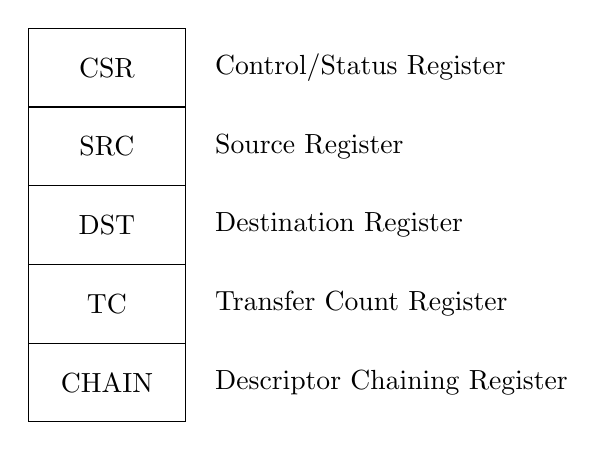
\begin{tikzpicture}
        \draw (0,0) -- (2,0) -- (2,-5) -- (0,-5) -- (0,0);

        \draw (0,-1) -- (2,-1);
        \draw (0,-2) -- (2,-2);
        \draw (0,-3) -- (2,-3);
        \draw (0,-4) -- (2,-4);

        \draw (1,-0.5) node[] {CSR};
        \draw (1,-1.5) node[] {SRC};
        \draw (1,-2.5) node[] {DST};
        \draw (1,-3.5) node[] {TC};
        \draw (1,-4.5) node[] {CHAIN};
    
        \draw (2.25,-0.5) node[right] {Control/Status Register};
        \draw (2.25,-1.5) node[right] {Source Register};
        \draw (2.25,-2.5) node[right] {Destination Register};
        \draw (2.25,-3.5) node[right] {Transfer Count Register};
        \draw (2.25,-4.5) node[right] {Descriptor Chaining Register};
    \end{tikzpicture}
\end{center}
\caption{DMA Controller Register Structure}
\label{fig:dma-reg}
\end{figure}


\subsubsection{DMA Chaining}
DMA's can be chained, this is were the descriptor points to a control block in memory. The control
block is loaded automatically by DMA chaining to start a DMA session. DMA chaining uses a linked
list structure. DMA chaining is shown in Figure \ref{fig:dma-chain}. As the values in the DMA
registers are memory mapped the DMA descriptors can be chained together with pointers. DMA chaining
can be use the achieve a ping pong buffer format, with the second DMA referring to the next buffer
and switching automatically once the transfer count is complete.

\begin{figure}[H]
\begin{center}
    \begin{tikzpicture}
        \draw (0,0) -- (2,0) -- (2,-5) -- (0,-5) -- (0,0);

        \draw (0,-1) -- (2,-1);
        \draw (0,-2) -- (2,-2);
        \draw (0,-3) -- (2,-3);
        \draw (0,-4) -- (2,-4);

        \draw (1,-0.5) node[] {CSR};
        \draw (1,-1.5) node[] {SRC};
        \draw (1,-2.5) node[] {DST};
        \draw (1,-3.5) node[] {TC};
        \draw (1,-4.5) node[] {CHAIN1};
    
        \draw (0,-6) -- (2,-6) -- (2,-11) -- (0,-11) -- (0,-6);

        \draw (0,-7) -- (2,-7);
        \draw (0,-8) -- (2,-8);
        \draw (0,-9) -- (2,-9);
        \draw (0,-10) -- (2,-10);

        \draw (1,-6.5) node[] {CSR};
        \draw (1,-7.5) node[] {SRC};
        \draw (1,-8.5) node[] {DST};
        \draw (1,-9.5) node[] {TC};
        \draw (1,-10.5) node[] {CHAIN2};

        % Draw Arrows
        \draw[arrow] (2,-2.5) -- (3,-2.5) |- (4,-0.5);
        \draw[arrow] (2,-8.5) -- (6.5,-8.5) |- (7,-0.5);

        \draw[fill=gray!10] (4,0) -- (6,0) node[above, midway] {Buffer 1} -- (6,-11) -- (4,-11) -- (4,0);

        \draw[fill=gray!10] (7,0) -- (9,0) node[above, midway] {Buffer 2} -- (9,-11) -- (7,-11) -- (7,0);

        \draw[arrow] (0,-4.5) -- ++(-0.5,0) |- (0,-6.5);
        \draw[arrow] (0,-10.5) -- ++(-1,0) |- (0,-0.5);

        \draw[arrow, line width=4pt] (-2,-1.5) -- (0,-1.5);
        \draw[arrow, line width=4pt] (-2,-7.5) -- (0,-7.5);
    \end{tikzpicture}
\end{center}
\caption{Two-Channel Double Buffered DMA Chaining}
\label{fig:dma-chain}
\end{figure}


\subsubsection{Ping-Pong Buffer}
The Ping Pong buffer, shown in Figure \ref{fig:ping-pong} is a simple buffering system that has two
buffers on the input and output of the processor. This arrangement maximises the processing efficiency
of the processor as data can always be made available and there is always a location to write output
data to.

\begin{figure}[H]
\begin{center}
\begin{adjustbox}{width=\textwidth}
    \begin{circuitikz}
        \draw[fill=red!10] (0,0) -- (2,0) -- (2,-2) -- (0,-2) -- (0,0);
            \draw (1,-1) node[] {\textbf{ADC}};

        \draw[fill=red!10] (3,0) -- (5.5,0) -- (5.5,-2.5) -- (3,-2.5) -- (3,0);
            \draw (4.25,-0.5) node[] {\textbf{BSP}};
            \draw[fill=blue!10] (3.5,-1) -- (5,-1) -- (5,-2) -- (3.5,-2) -- (3.5,-1);
            \draw (4.25, -1.5) node[] {DRR};

        \draw[fill=red!10] (6.5,0) -- (8.5,0) -- (8.5,-2.5) -- (6.5,-2.5) -- (6.5,0);
            \draw(7.5,-1.25) node[] {\textbf{DMA}};

        \draw[fill=red!10] (19,0) -- (21,0) -- (21,-2) -- (19,-2) -- (19,0);
            \draw (20,-1) node[] {\textbf{D/A}};

        \draw[fill=red!10] (15.5,0) -- (18,0) -- (18,-2.5) -- (15.5,-2.5) -- (15.5,0);
            \draw (16.75,-0.5) node[] {\textbf{McBSP2}};
            \draw[fill=blue!10] (16,-1) -- (17.5,-1) -- (17.5,-2) -- (16,-2) -- (16,-1);
            \draw (16.75, -1.5) node[] {DXR};

        \draw[fill=red!10] (12.5,0) -- (14.5,0) -- (14.5,-2.5) -- (12.5,-2.5) -- (12.5,0);
            \draw(13.5,-1.25) node[] {\textbf{DMA2}};


        \draw[fill=gray!30] (3,-4) -- (5,-4) -- (5,-6) -- (3,-6) -- (3,-4);
            \draw[text width=2cm, text centered] (4,-5) node[] {PING IN};
        \draw[fill=gray!10] (3,-7) -- (5,-7) -- (5,-9) -- (3,-9) -- (3,-7);
            \draw[text width=2cm, text centered] (4,-8) node[] {PONG IN};
        
        \draw[fill=gray!30] (16,-4) -- (18,-4) -- (18,-6) -- (16,-6) -- (16,-4);
            \draw[text width=2cm, text centered] (17,-5) node[] {PING OUT};
        \draw[fill=gray!10] (16,-7) -- (18,-7) -- (18,-9) -- (16,-9) -- (16,-7);
            \draw[text width=2cm, text centered] (17,-8) node[] {PONG OUT};

        \draw[fill=red!10] (9,-5.5) -- (12,-5.5) -- (12,-7.5) -- (9,-7.5) -- (9,-5.5);
            \draw (10.5,-6.5) node[] {Processing};
            \draw (10.5,-5.5) node[above] {\textbf{CPU}};
        
        % Switches
        \draw[/tikz/circuitikz/bipoles/length=4cm] (1,-6.5) node[spdt] (insw0) {};
        \draw (insw0.out 1) -- ++(0.3115,0);
        \draw (insw0.out 2) -- ++(0.3115,0);

        \draw[/tikz/circuitikz/bipoles/length=4cm] (7,-6.5) node[rotate=180, spdt] (insw1) {};
        \draw (insw1.out 1) -- ++(-0.3115,0);
        \draw (insw1.out 2) -- ++(-0.3115,0);
        \draw (9,-6.5) -- (insw1.in);
        
        \draw[/tikz/circuitikz/bipoles/length=4cm] (14,-6.5) node[spdt] (outsw0) {};
        \draw (outsw0.out 1) -- ++(0.3115,0);
        \draw (outsw0.out 2) -- ++(0.3115,0);
        \draw (12,-6.5) -- (outsw0.in);

        \draw[/tikz/circuitikz/bipoles/length=4cm] (20,-6.5) node[rotate=180, spdt] (outsw1) {};
        \draw (outsw1.out 1) -- ++(-0.3115,0);
        \draw (outsw1.out 2) -- ++(-0.3115,0);

        % Arrows
        \draw[arrow] (2,-1.5) -- (3.5,-1.5);
        \draw[arrow] (5,-1.5) -- (6.5,-1.5);
        \draw (7.5,-2.5) |- (-2,-3) |- (insw0.in);
        \draw (outsw1.in) -| (23,-3) -| (13.5,-2.5);
        \draw[arrow] (14.5,-1.5) -- (16,-1.5);
        \draw[arrow] (17.5,-1.5) -- (19,-1.5);
    \end{circuitikz}
\end{adjustbox}
\end{center}
\caption{Ping Pong Buffer Configuration}
\label{fig:ping-pong}
\end{figure}

